\section*{Appendix}

%%%%%%%%%%%%%%%%%%%%%%%%%%%%%%%%%%%%%%%%%%%%%%%%%%%%%%%%%%%%%%%%
% DATASETS
%%%%%%%%%%%%%%%%%%%%%%%%%%%%%%%%%%%%%%%%%%%%%%%%%%%%%%%%%%%%%%%%
\section{Datasets}
    \subsection{VQA-CP}
    VQA-CP (Visual Question Answering under Changing Priors)~\cite{vqa-cp} is a re-organization of the VQA dataset~\cite{antol2015vqa,goyal2017making}.
    The aim of VQA-CP is to have a different distribution of answers per question type is different in test and train splits.
    There are 65 question types based on the prefix of the questions such as \textit{``how many", ``what color", ``what sport", ``is there", "what is the", ``which"}.
    In VQA-v2, samples are drawn at randomly and independently and assigned either to train or test, thus resulting in the same distribution for both splits.
    \begin{equation*}
        P^{VQA}_{train}(A | Q, I) = P^{VQA}_{test}(A | Q, I).
    \end{equation*}
    
    In VQA-CP however, samples are assigned using a greedy re-splitting algorithm,  either to train or test, in a way that makes sure that questions with the same type an same answer are not shared by train and test.
    It is important to note that there is no leakage between train and test splits compared to the original VQA splits.
    \begin{equation*}
        P^{VQA-CP}_{train}(A | Q, I) \neq P^{VQA-CP}_{test}(A | Q, I).
    \end{equation*}
    
    The train set for VQA-CP-v2 contains 121k images, 245k questions and 2.5M answers, while the test set contains 98k images, 220k questions and 2.2M answers.
    
    \subsection{COCO}
    The source of images in both VQA and VQA-CP is the MS-COCO dataset~\cite{lin2014microsoft}.
    COCO contains natural images representing complex, real-world scenes containing common objects of 91 categories such as \textit{``person", ``chair", ``fork", ``horse", ``sports-ball"}, etc.
    For each image, COCO provides 5 captions along with bounding boxes and polygon annotations for each object instance in the image.
    

%%%%%%%%%%%%%%%%%%%%%%%%%%%%%%%%%%%%%%%%%%%%%%%%%%%%%%%%%%%%%%%%
% IMAGE MUTATION PROCESS
%%%%%%%%%%%%%%%%%%%%%%%%%%%%%%%%%%%%%%%%%%%%%%%%%%%%%%%%%%%%%%%%
\begin{figure}[t]
    \centering
    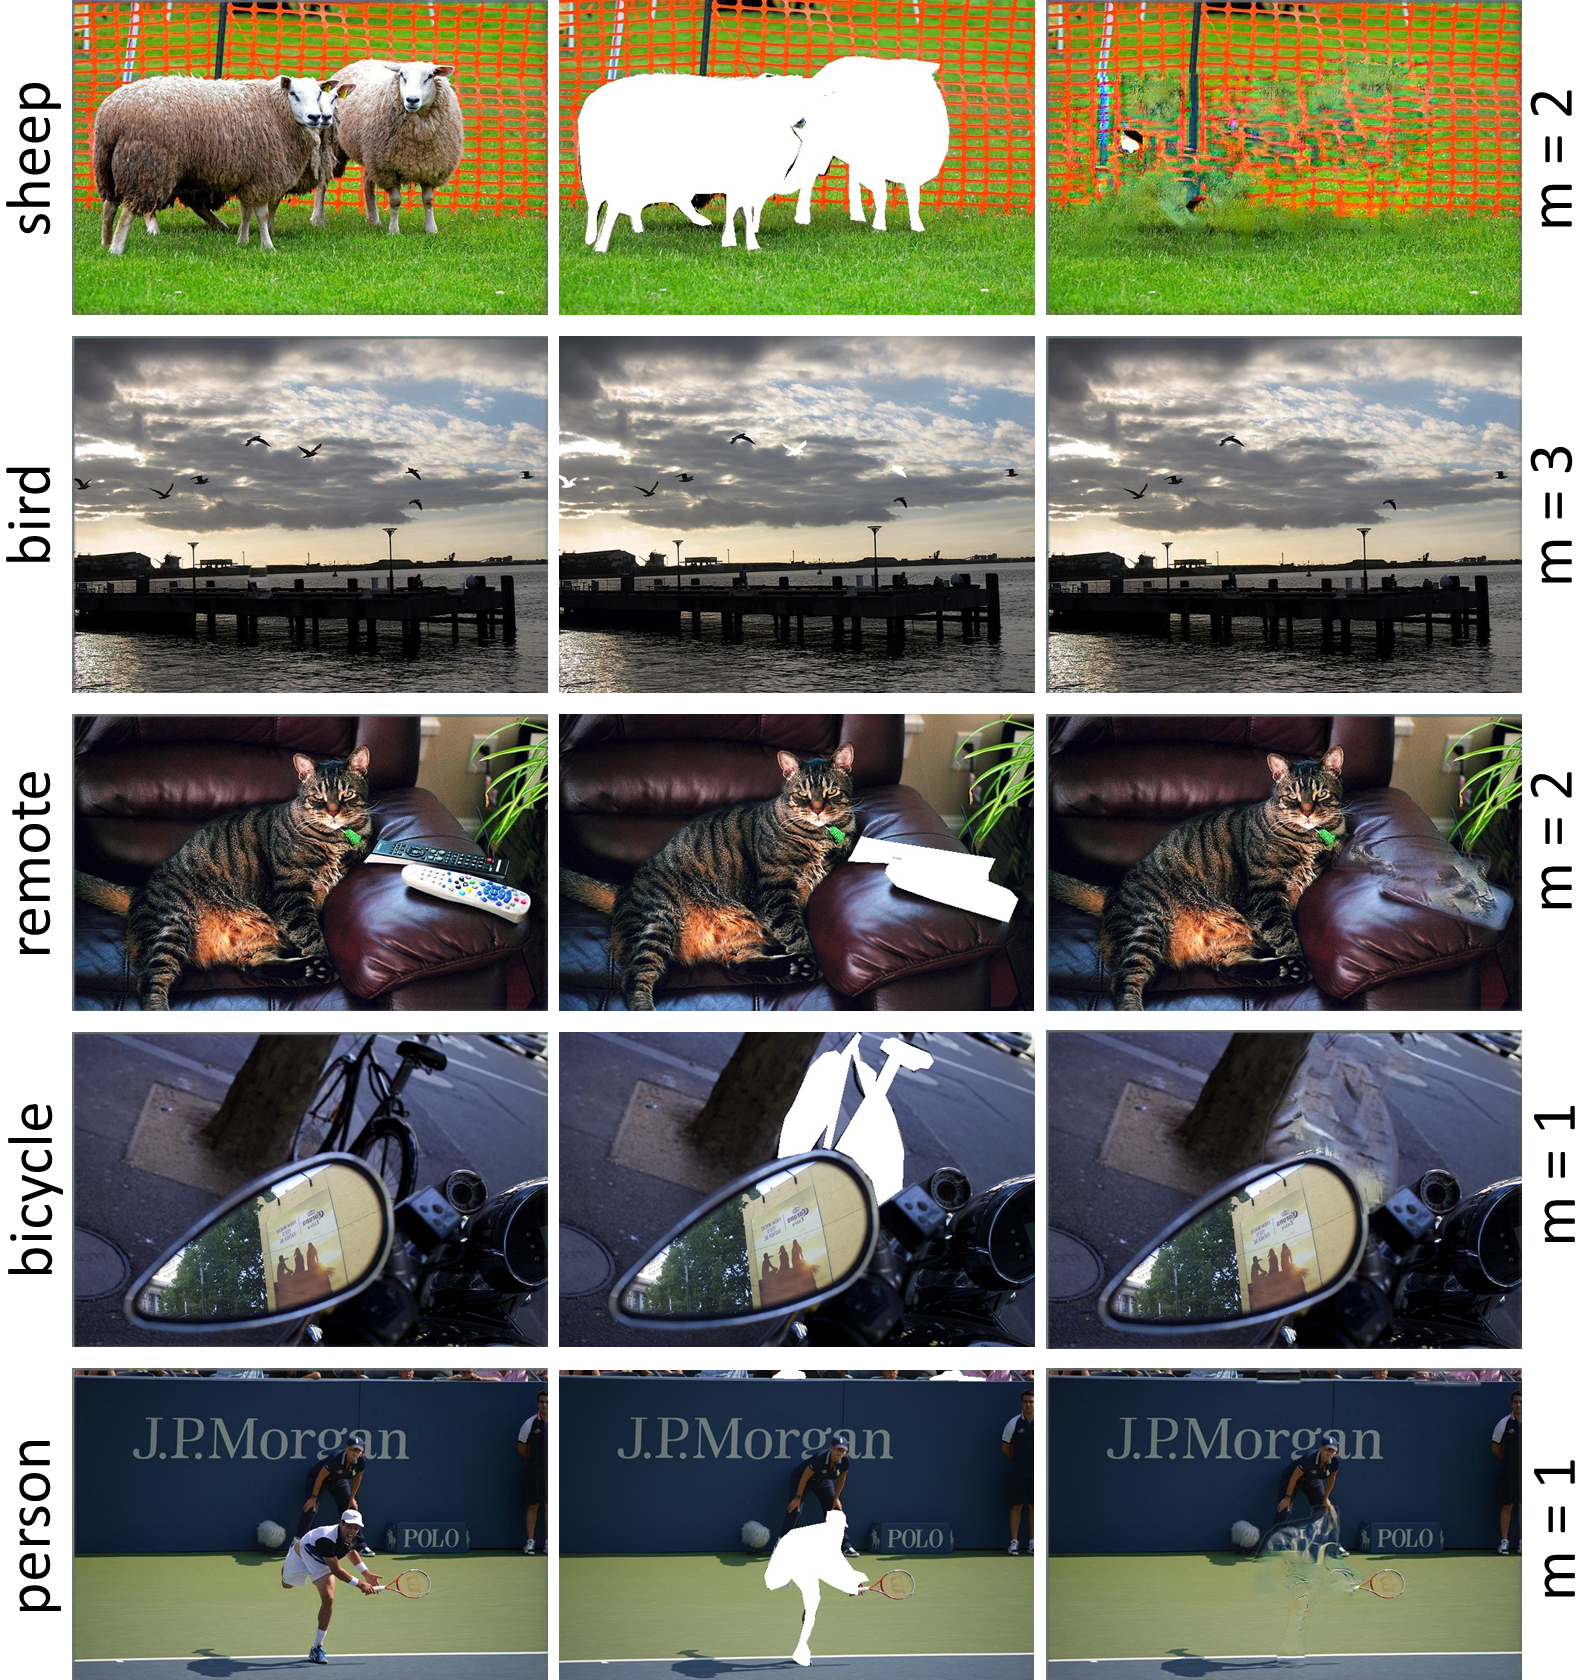
\includegraphics[width=\linewidth]{ figures/supp_inp.pdf}
    \caption{Illustration of COCO bounding box and polygon annotations for $m$ instances of an object, and the inpainting results after removal}
   
    \label{fig:bbox}
\end{figure}


\begin{figure}[t]
    \centering
    \includegraphics[width=\linewidth]{ figures/supp_col.pdf}
    \caption{Illustration of color inversion procedure}
    \label{fig:col}
\end{figure}

\section{Image Mutant Generation Process}
    
In this section we provide additional details about our process for generating mutant samples from original question-image-answer triplets (Q-I-A) in the VQA-CP dataset.
For all linguistic operations we use a combination of SpaCy~\cite{honnibal2017spacy} and the LemmInflect library~\cite{lemminflect}
% \footnote{{\url{ https://github.com/bjascob/LemmInflect}}} 
for lemmatization and inflection.

    
    \subsection{Selection of Objects}
    For each VQA sample, a list of words $W$ is created, which contains words from the ground-truth answers and the question.
    All nouns in $W$ are converted to their singular form.
    For yes-no questions, numeric questions, and questions about colors of objects, a list of objects $O$ is obtained from COCO.
    Background and crowd objects are filtered out from $O$.
    From $O$ critical objects $O_C$ and and non-critical objects $O_{NC}$ are obtained.
    Critical objects are those objects in the image that when manipulated or removed, may change the answer to the question being asked.
    For this we follow a simple heuristic that states that if an object-word or it's synonym or hyponym is present in $W$, then it is a critical object.
    Then a critical object $o \in O$ is chosen at random, and $m$ instances of this object are chosen at random.
    The polygon annotations (a polygon border) for this object are obtained from the COCO dataset as shown in Figure~\ref{fig:bbox}.
    Using these annotations, either a removal or color-inversion operation is applied to create the mutant image.
    
    
    \subsection{Object Removal and In-painting}
    After the object instance is selected, it is removed from the image by replacing all pixel values by 1 (white).
    This masked image is then input to a GAN-based image inpainting network~\cite{yu2018generative} that fills up this pixels in the mask.
    This makes the image photorealistic.
    This network is one of the best available off-the-shelf blind image inpainting models, and is trained on the ImageNet~\cite{deng2009imagenet}.
    The masked image could also be used as the mutant image however we prefer to use photorealistic images for two main reasons.
    First, masked images do not lie in the same distribution as natural images, and secondly, the mask boundary may give clues to the network about the the shape or outline of the missing object.
    
    
    \subsection{Color Inversion Process}
    For mutation that involves a change in the color of the object, we perform a simple pixel-wise color inversion operation on each pixel in the mask to get the mutant image as shown in Figure~\ref{fig:col}.
    This is to ensure that we do not use any prior knowledge about valid colors of a specific object.
    For instance, bananas can typically be yellow, green, or black. 
    However, if we only change the color or a banana to one of these three colors, we would be using domain knowledge and inadvertently introducing answers from the test set, defeating the purpose of OOD generalization.
    Although the simple inversion process can introduce unnatural colors like blue bananas, it forces the model to understand colors in the image to answer the question instead of simply answering from linguistic priors (such as the memorized knowledge that bananas can be green, yellow, or black).
    
    
    \subsection{Answer Generation}
    The new answers are generated based on the type of question.
    For \textbf{yes-no questions}, if all instances of the object are removed then the answer changes from yes to no. 
    If only some instances are removed or if the object is non-critical, the answer remains the same.
    For \textbf{number questions}, if $m$ instances of a critical object are removed, the answer changes from $n$ to $n-m$, else the answer remains the same.
    For \textbf{color-based questions} we convert the answer color to their HEX value using Webcolors \footnote{\url{https://pypi.org/project/webcolors/}}, invert the value, and find the color in CSS-21 colors closest to this value to generate the new answer.
       
%%%%%%%%%%%%%%%%%%%%%%%%%%%%%%%%%%%%%%%%%%%%%%%%%%%%%%%%%%%%%%%%
% QUESTION MUTATION PROCESS
%%%%%%%%%%%%%%%%%%%%%%%%%%%%%%%%%%%%%%%%%%%%%%%%%%%%%%%%%%%%%%%%    

\begin{table}
    \centering
    \resizebox{\textwidth}{!}{
    \begin{tabular}{@{}lllll@{}}
        \toprule
        \textbf{Mutation} & $\mathbf{Q}$ & $\mathbf{A}$ & $\mathbf{Q_{mutant}}$ & $\mathbf{A_{mutant}}$ \\
        \toprule
        \multirow{4}{*}{Negation} & Is this bread? & yes & Is this not bread & no \\
         & What is the color of the woman's shirt? & black & What is not the color of the woman's shirt? & white\\
         & Are there deciduous trees? & no & Are there no deciduous trees? & yes \\
         & Is there a boy? & no & Is the no boy? & yes \\
        \midrule
        \multirow{3}{*}{Adversarial} & Who is riding the boat? & man & Who is riding the desk & \textit{``can't say"}\\
         & How big is the plane? & large & How big is the book? & \textit{``size"} \\
         & How many pillows are on the bed? & four & How many pillows are on the table? & \textit{``number"} \\
        \midrule 
        \multirow{4}{*}{Masking} & What type of drink is being displayed? & wine & What type of [MASK] is being displayed? & \textit{``beverage"} \\
         & How many bins? & two & How many [MASK] ? & \textit{``number" }\\
         & What is the green stuff on the sandwich? & lettuce & What is the green stuff on the [MASK]? & \textit{``food"} \\
        \bottomrule
    \end{tabular}
    \caption{Examples of three types of question mutation with new answers}
    \label{tab:negation}
    }
\end{table}
\begin{table*}[H]
    \centering
    \small
    % \resizebox{\linewidth}{!}{
    \begin{tabular}{@{}ll @{}}
        \toprule
        \textbf{Category} & \textbf{Member Answers}\\
        \toprule
        time of day & afternoon, dusk, sunset, sunrise, night, daytime, evening, morning, dawn\\
        weather     & rainy, sunny, snowing, cloudy, windy, storm, blurry, fog, dust-storm, tornado \\
        action      & playing, cutting, talking, dancing, singing, hugging, waving, working, standing, sitting \\
        emotion     & angry, curious, tired, happy, bored, surprise, confused, sad \\
        furniture   & table, chair, desk, couch, sofa, bed, ottoman, barstool, seat, bench \\
        material    & granite, wood, brick, glass, stone, oak, concrete, asphalt, plaster \\
        country     & taiwan, france, canada, indonesia, australia, india, britain, hong kong \\
        person      & man, woman, child, kid, boy, people, baby, lady, girl, adult, male, female, players \\
        \bottomrule
    \end{tabular}
    % }
    \caption{Examples of answer categories and member answers per category}
    \label{tab:categories}
\end{table*}
\begin{figure*}[t!]
    \centering
    \includegraphics[width=\linewidth]{ figures/a_distrib.png}
    \caption{The distribution of answers by question types for VQA train and Mutant compared with VQA-test}
    \label{fig:a_distrib}
\end{figure*}


\section{Question Mutant Generation Process}
For generating question mutants, we use three operators: negation, substitution by antonyms or adversarial words, and masking critical words. 

    \subsection{Negation}
    
    For yes-no questions and color-based questions, we use a template-based negation technique that puts a negative word such as \textit{``not"} or \textit{``no"} before a preposition, noun phrase, or verb.
    For instance ``Is this chair broken?" is negated to ``Is this chair not broken?".
    We show examples of negation in Table~\ref{tab:negation}.
    Negation simply flips the answer from yes to no or no to yes.
    
    \subsection{Adversarial Words and Masking}
    Another form of question mutation is substituting object-words with their adversarial words.
    To do so, we create a list of all object words and their synonyms and use BERT~\cite{devlin2018bert} similarity to rank the most similar words.
    To replace a word, we chooser the most similar word which is not present in the image.
    The third type of mutation is masking, where a critical object word is removed from the question and replaced with the token ``MASK".
    
    For both these types of mutations, determining the correct answer in some cases is not possible as can be seen from examples in Table~\ref{tab:negation}.
    Thus we use the broad category as the answer. 
    For instance, when a question such as \textit{``How big is the book"} is replaced with either \textit{``How big is the plane"} or \textit{``How big is the [MASK]"}, it is clear that the question is about the size of an object.
    Thus we annotate this question with this broad category ``size" as the answer.
    In other cases, where even a broad category cannot be ascertained, the answer is replaced with ``can't say" or "don't know".
    



    To generate answer clusters and representative answer categories, we extract Glove~\cite{pennington2014glove} word vectors for each answer phrase/word using Spacy. 
    We use k-means clustering~\cite{lloyd1982least} with Euclidean distance metric and with varying number of $K$. 
    We manually tune the number of clusters till we observe a clear set of categories appear at $K=50$.
    We then manually annotate the category names.

%%%%%%%%%%%%%%%%%%%%%%%%%%%%%%%%%%%%%%%%%%%%%%%%%%%%%%%%%%%%%%%%
% STATISTICS
%%%%%%%%%%%%%%%%%%%%%%%%%%%%%%%%%%%%%%%%%%%%%%%%%%%%%%%%%%%%%%%%    

\section{Dataset Analysis}
Here we provide dataset analysis in terms of distribution of answers by question-type, number of samples for each type of mutation, and the final distribution of the dataset in terms of answer-type.

\begin{table}[t]
    \centering
    \small
    \begin{tabular}{| c | c | c |}
        \hline
        \textbf{Category} & \textbf{VQA-CP (\%)} & \textbf{Mutant (\%)}\\
        \hline 
        Yes/No & 41.86 & 47.88 \\
        Number & 11.91 & 13.64 \\
        Other  & 46.23 & 38.48 \\
        \hline
    \end{tabular}
    \caption{Distribution of samples in the dataset by answer type}
    \label{tab:ans_type}
\end{table}
    \subsection{Distribution by Question Type}
    We show the distribution of answers per question type in Figure~\ref{fig:a_distrib} for three categories \textit{``How many", ``What sport", and ``What color"} for the top-10 answers.
    It can be seen that the distribution is distinct from the test data and close to the VQA-CP train data apart from the introduction of categorical answers such as \textit{``number" and ``sports"} during question mutation.
    Our mutation method does not leak information about answers from test set to train set.

        \begin{table}[t]
    \centering
    \small
    \begin{tabular}{@{}cc@{}}
        \toprule
        \textbf{Mutation Category} & \textbf{Number of Samples}\\
        \toprule
        Object Removal  & 159,899\\
        Color Change    & 30,759 \\
        Negation        & 237,611 \\
        Adversarial Substitution & 146,814 \\
        Word Masking & 104,666\\
        \bottomrule
    \end{tabular}

    \caption{Distribution of generated mutant samples by category of mutation}
    \label{tab:mutant_type}
\end{table}



    \subsection{Distribution by Mutation Type}
    Table~\ref{tab:mutant_type} shows the number of samples generated by each type of mutation.

    
    \subsection{Distribution by Answer Type}
    There are three answer types in both VQA-CP and Mutant datasets: \textit{yes/no, number, and other}.
    Creation of mutant samples leads to a small change in the distribution as shown in Table~\ref{tab:ans_type}.
